\documentclass[11pt, a4paper]{article}
\usepackage{graphicx}
\title{AudioScout\texttrademark{} : Audio Content Indexing Software\footnote{doc version 1.0.0}}
\author{Aetilius, Inc.}
\date{October, 2010}
\begin{document}
\maketitle

\section{Overview}
\paragraph{AudioScout\texttrademark{} is a distributed content indexing system. It can index a
large collection of audio content for the purpose of later recognition of unknown signals. 
Robust to noise, different encodings and other types of distortion, it can be used 
for a variety of applications including duplicate detection of files as well as more sophisticated  
uses involving the enforcement of copyrights and lawful use.}    

\paragraph{The AudioScout\texttrademark{} system is a collection of servers that manage the storage and matching of 
audio signals in a large body of audio content.  When new audio signals are added 
to the index, a compact hash is calculated based on low-level signal features.  This hash  serves as a temporal description of 
the signal.  The hash values are then  added as entries into one of the distributed tables.  AudioScout additionally stores 
meta  information associated with that signal into a database for later retrieval.  For queries of unknown signals, its 
perceptual  hash  must be calculated in order to find the matching signal in the table and retrieve the associated metadata.}
 
\section{Features}
\flushleft
\begin{itemize}
\item[*] Able to build index files during normal server operation; can start new 
table servers or terminate them at any time without effecting operation of the main server.
\item[*] Make online additions to the table server through the auscoutd front end server, as well
as the use of a utility program to build the index tables locally.
\item[*] Ability to hash any part of an unkown signal and perform a lookup on that signal. As
long as the portion being hashed was previously added to the index, AudioScout should find
the matching signal.   
\item[*] System can scale to a large number of tables over a network  of machines.
\item[*] Separate database server providing multi-threaded access to sqlite database 
for storage of related file meta data; can be run on any machine in the network.
\item[*] Simple to set up and use.  Various client applications can be easily created to query 
and add to the index. 
\item[*] Complete system logging integration (syslog) with eight log levels.
\item[*] Relatively small memory footprint and fast operating time.
\end{itemize}

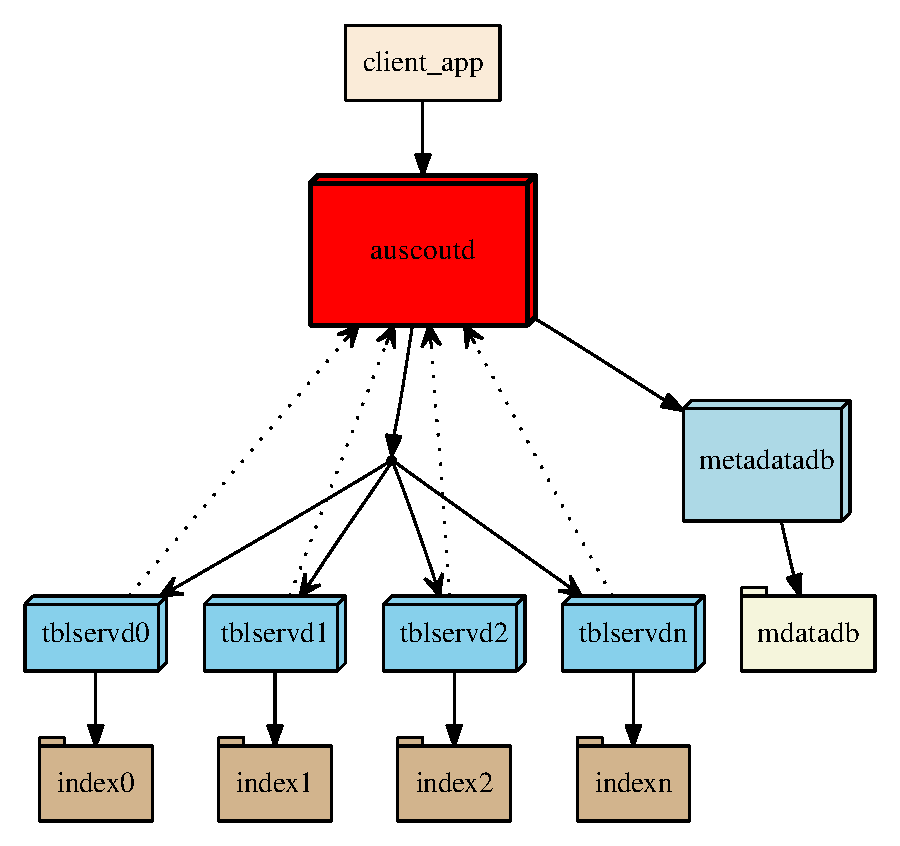
\includegraphics{audioscout.eps}
\newpage

\section{Architecture}
\paragraph{The AudioScout central server manages the storage of perceptual hashes in the distributed table
servers along with the storage and retrieval of metadata information.  A perceptual hash is a 
compact temporal description of a signal's low level frequency characteristics. Audio Scout uses a
perceptual hash algorithm to extract such a characterization from  each signal.  Matches are 
found by publishing the hash 
of the query signal to all the available table servers.  Each table server tries to 
determine the unique id that is matched most often to the sequence and sends it back to the main 
server.  The main server can then use this id to retrieve that entries' metadata from the metadata 
database server.}

\subsection{AudioScout Server}
\paragraph{This is the main server providing the ability to add new audio signals to the index as well as 
the ability to perform queries for the identification of unknown content.  The server is a multi-
threaded process servicing client requests in two modes: query and insertion. In query mode,
 the main server publishes the recieved hash to its network of table servers and waits for the 
result.  If a match is found, the audio scout server recieves the unique id of the match from one
of the table servers, and then, using this id, it retrieves the correct information from the 
metadata server for return to the client application.  If not found, an empty message is
 returned.  
For insertions, a particular table is randomly chosen from the list of available servers, and 
the hash is published for that table to add to its index.  The meta information which is included 
with the hash from the client application is stored in the metadata server.  The unique id for 
that entry is returned to the client application.  However, the source of that metadata is not 
strictly tied to the contents of the file;  other client applications can easily be created 
to gather such information from other sources.}

\subsection{Distributed Table Servers}
\paragraph{Each table server provides access to an associated file index of hash entries.  Since hashing all 
audio files into an index can involve a very time consuming process - especially for hundreds, 
thousands or even millions of files - this distributed approach allows for concurrently building 
separate index files on any number of host machines.  The size of each index file is only limited 
by the host machine's memory limitations.  For this initial process of building the index,  a 
utility program is provided to read the audio files, hash the files 
and then add them to the index.}
\paragraph{Once the index is built, the table servers can be started for 
each of these index files.  Additional insertions can always be done through the main audio scout 
server interface or by termination of the server and adding to the index with the utility program.
While terminating the table server does disable queries against that particular index's entries, 
it does not effect the overall operation of the system.}
\paragraph{It is important to note that new entries added through the 
audio scout server are not immediately added to the index, but are inserted into a temporary 
index file that can later be merged into the main index file.  The Audio Scout system has 
included a simple means to merge the tables by sending user signals to the table server, 
which can conveniently be scheduled as a cron task. For this reason, new additions to the index
are not immediately available, but must wait for the next merge operation.  The reasons for this
feature are twofold: (1) the index table used is a memory mapped file and is not accessible for
write operations.  The table must be closed and reopened in write mode, and (2)
 since deletions of entries is a tedious process, this can provide a
filtering layer to the addition of new signals to ensure only legimate files are added.}
  
\subsection{MetaDataDB Server}
\paragraph{The metadata server is a multi-threaded process that is a wrapper around a sqlite database for 
all the metadata. It operates in two modes: insertion of new entries and query 
by a unique id. It is meant to serve requests by the audio scout server, but it also 
allows convenient access to metadata through the sqlite utilities.}
\newpage
\section{Public API}
The public interface to the auscoutd server is very simple and easy to use.  
It can be accessed by the following multi-part zeromq message.\\
\vspace{5mm}
\fbox{ cmd | nbframes | hash array | metadata string}\\
\vspace{5mm}
cmd - (uint8) represents mode (cmd = 1 for query, cmd = 2 for submission).\\
nbframes - (uint32) represents length of the hash array.\\
hash - (uint32 array) represents the perceptual hash to send.\\
\vspace{5mm}
The metadata string is only for user submissions (cmd = 2) and can be formed with 
the following fields,  each field seperated by the ascii record separator character, RS 
(or 30 in decimal). Each 
field is a string unless otherwise noted.\\
\vspace{5mm}
\fbox{composer|title|performer|date|album|genre|year (int)|duration (int) |part of set (int)}
\vspace{5mm}

All multi-byte variables are serialized to little-endian format for transmission over the
network.

\section{Installation and Set Up}
The audio scout servers are quite easy to set up.  Here is a general outline of the process:
\begin{enumerate}
\item Create metadata sqlite database with the included sql schema.  
\item Start metadatadb server on a particular host machine with the sqlite database. 
\item Build the index files. This can be done with the audioindex utility file.  If an index is 
not built, a table server may be started and an empty index will be created.  
Insertions can then be made with the audio scout server interface.  
\item Start AudioScout server with the address of the metadatadb server.
\item Start Table Server for each audio index file. It must be given the address and port for
where to find the audio scout main server in order to register and send back results.  
\item Start the client application to index new signals or perform queries for unknown signal
content. Currently, there is a simple console application. Fuller featured client applications
can be easily created.
\end{enumerate}

\section{Tests}

\subsection{tblservd tests}
To get a sense of the throughput capabilities of the system, the following test was performed 
on the table server component\footnote{This test was performed on Intel Pentium IV 1GHz 
processor}, since that is, in fact, where the bulk of the work is done.  
The first two graphs below reveal system limits across a varying number of worker threads running 
in the table server. The first one shows maximum response times when 100 queries flood the table 
server at five different levels of arrival rates.  The maximum time in each case is the response time for 
the query that is at the end of the longest queue that forms.  The second graph shows the 
corresponding recieve-to-send rate ratios for each number of worker threads.  This ratio is 
calculated by the rate queries are sent divided by the rate at which the results are recieved.  
Each rate is the total number of queries per second. The ratio itself is a measure of the 
clearing ability of the table server. In other words, values closer to one mean greater ability 
for the system to service queries without a queue forming. In this case,  it is clear that 
the increases in performance tend to level off at around 
50 threads.
 
\includegraphics[angle=-90,width=\linewidth]{tblperfthreads.eps}

The next two graphs below show the same behavior for a fixed number of worker threads (60) 
and a varying number of total queries.  The data is taken for three different 
query rates - 100, 200 and 1000 queries/second.   Notice how the table server can easily 
handle both 100 and 200 queries/second for up to around 50 queries before a queue forms.  
Even so,  it seems the table server can still handle larger bursts at these rates. 
For example, the maximum response time does not grow to over 5 seconds until around 200 queries 
have been submitted.

\includegraphics[angle=-90,width=\linewidth]{tblperfthruput.eps}

\subsection{metadatadb Tests}
The performance tests on the metadatadb server were conducted by extracting the metadata 
from a large corpus of audio files and submitting them to the server at given query rates,
measured in queries per second.  The first two plots show the average response rates and the
effective query rate for different inter-arrival times between the delivered queries. As can
be seen in the plot, the average response time remains quite constant across all query rates,
and the plot of the effective query rate increases as the inter-arrival time between queries is
reduced. Notice how the effective query rate reaches a maximum of around 250 queries per second 
when the queries immediately succeed one another.

\includegraphics[angle=-90,width=\linewidth]{mdperfthruput.eps}

In order to increase the query submission rate to above that which is permitted by simply 
reducing the inter-arrival time to 0 ms, the test driver program was designed to include multiple
threads from which to submit queries to the metadatadb server.  The driver program extracts the 
metadata from all the audio files and passes each thread a portion of submissions to submit to 
the server for inclusion into the database.  The next two plots reveal response times and
effective query rates for various numbers of these submission threads in the driver program. The
number of threads in the server is kept to a constant one and the inter-arrival time of queries is
kept to 0 ms.  Notice where the average response time slowly climbs 0.200, as the number of driver
threads is increased, and the effective query rate remains relatively constant (with some 
statistical fluctuations).

\includegraphics[angle=-90,width=\linewidth]{mdperfthreads.eps}

On the other hand, the number of threads in the metadatadb server appears to have little effect
on either the query rate or the average response rate, as shown in the next two graphs.

\includegraphics[angle=-90,width=\linewidth]{mdperfthreads2.eps}

\section{Dependencies}
\begin{itemize}
\item[--] zeromq version 2.0.9 www.zeromq.org/
\item[--] sqlite3 version 3.6.23.1  www.sqlite.org/
\item[--] libsndfile version 1.0.21 www.mega-nerd.com/libsndfile/
\item[--] libsamplerate version 0.1.7 www.mega-nerd.com/SRC/
\item[--] libmpg123 version 1.12.1 www.mpg123.de/api (for mp3 file support)
\end{itemize}
\section{Contact}
\begin{itemize}
\item D. Grant Starkweather dstarkweather@phash.org\\
\item Evan Klinger  eklinger@phash.org\\
\end{itemize}

\end{document}
